One question arises while mapping electrodes is that what should be the orientation of the active marker? but recall that we are only interested in the tip position of the marker which is independent of the orientation. However, we tried to evaluate the positional error by measuring the same electrode with 10 different orientation of the active marker. 

\begin{figure}[hbt!]
	\centering
	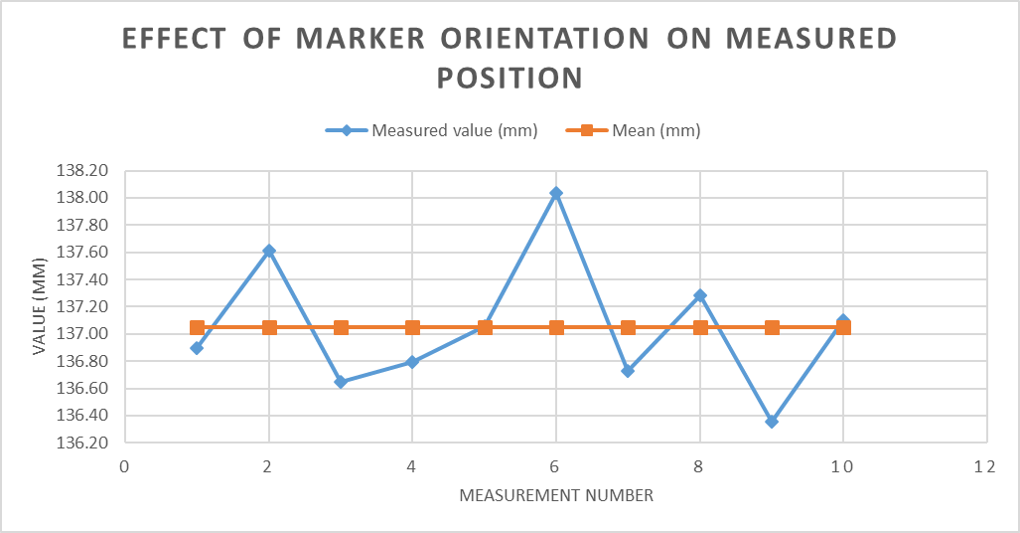
\includegraphics[scale=0.8]{active_marker_positional_error_normalised.png}
	\caption{Normlised positional error with 10 different orientation of active marker} 
	\label{fig:active_marker_normalised_positional_error}
\end{figure}


\cref{fig:active_marker_normalised_positional_error} shows the normalised values of positional errors due for 10 different marker orientation, although error along $\vect{X}$ , $\vect{Z}$ axis are small it is worth while to notice $\pm15\%$ error along $\vect{Y}$ axis.


Recall that we had to disturb the head position in order to map all the electrodes and we did it by introducing a common frame of reference i.e. robots end-effector frame. But this also comes with a cost and results in a positional error we also evaluated the positional error due to rotating head along a single axis and multiple axes to cover all electrodes. First, we rotated the phantom head to 10 different angles along a single axis while measuring the position of the single electrode at each of these 10 angles. Then, we repeated the same procedure but moved the phantom head along multiple axes and the positional error is recorded. 

\begin{figure}[hbt!]
	\centering
	\begin{subfigure}{0.49\textwidth}
		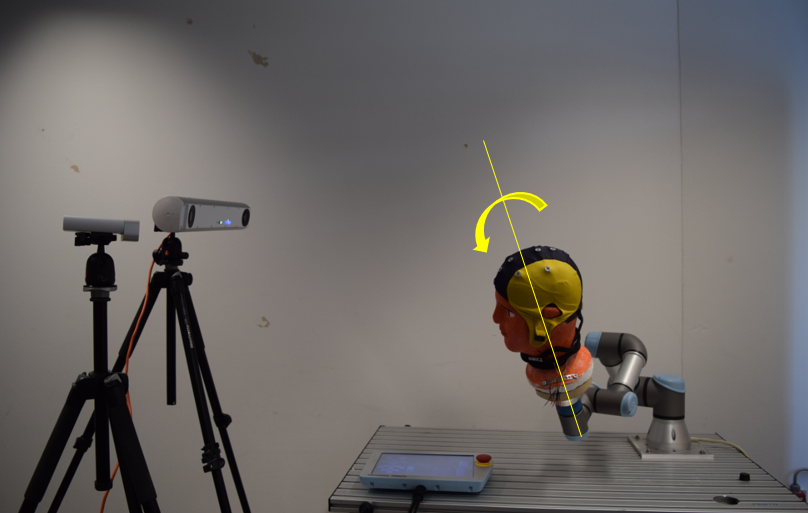
\includegraphics[width=\textwidth]{phantom_single_axis.png}	
	\end{subfigure}
	\hfill
	\begin{subfigure}{0.49\textwidth}
		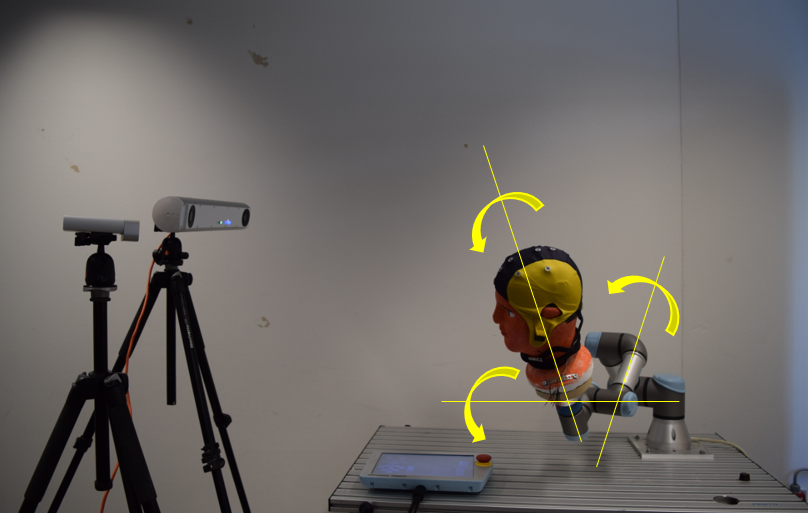
\includegraphics[width=\textwidth]{phantom_multiple_axis.png}	
	\end{subfigure}
	\caption{Rotating phantom head along single and multiple axis} 
	\label{fig:phantom_multiple_axis}
\end{figure} 

\begin{figure}[hbt!]
	\centering
	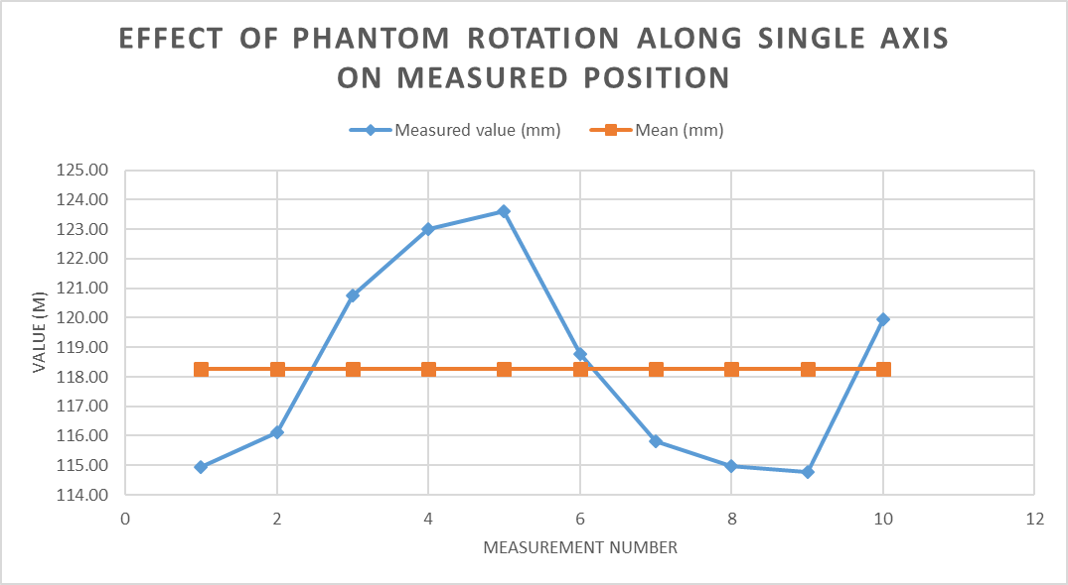
\includegraphics[scale=0.8]{normalised_positional_error_single_axis.png}
	\caption{Normlised positional error with phantom head roatated to 10 different angle along an axis.} 
	\label{fig:Normalised_positional_error_single_axis}
\end{figure}

\begin{figure}[hbt!]
	\centering
	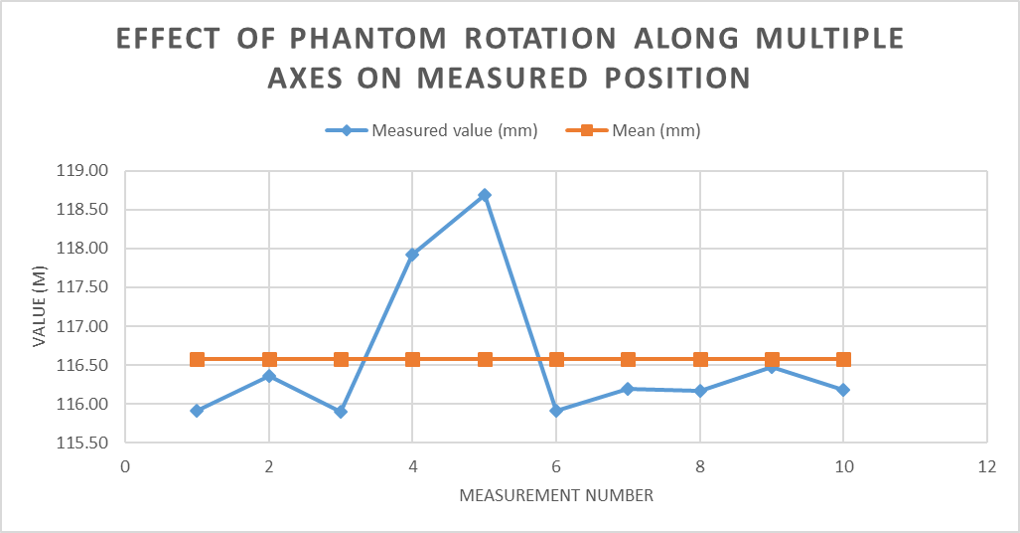
\includegraphics[scale=0.8]{normalised_positional_error_multiple_axis.png}
	\caption{Normlised positional error with phantom head roatated to 10 different position along multiple axis.}  
	\label{fig:Normalised_positional_error_multiple_axis}
\end{figure}

\cref{fig:Normalised_positional_error_single_axis} and \cref{fig:Normalised_positional_error_multiple_axis} shows the normalised values of positional errors due to the movement of the phantom head along single and multiple axes respectively. The combination of marker orientation with phantom movement along a single axis resulted in an error of $\pm10\%$ while along multiple axes it is little under $\pm7\%$. 



All the 22 electrodes are mapped to head coordinate system and their posotion is plotted in the \cref{fig:electrodes_blue_cap_1}. \cref{fig:electrodes_blue_cap_1_side_view} shows the side views for clear understanding of distribution of the electrodes.

\begin{figure}[hbt!]
	\centering
	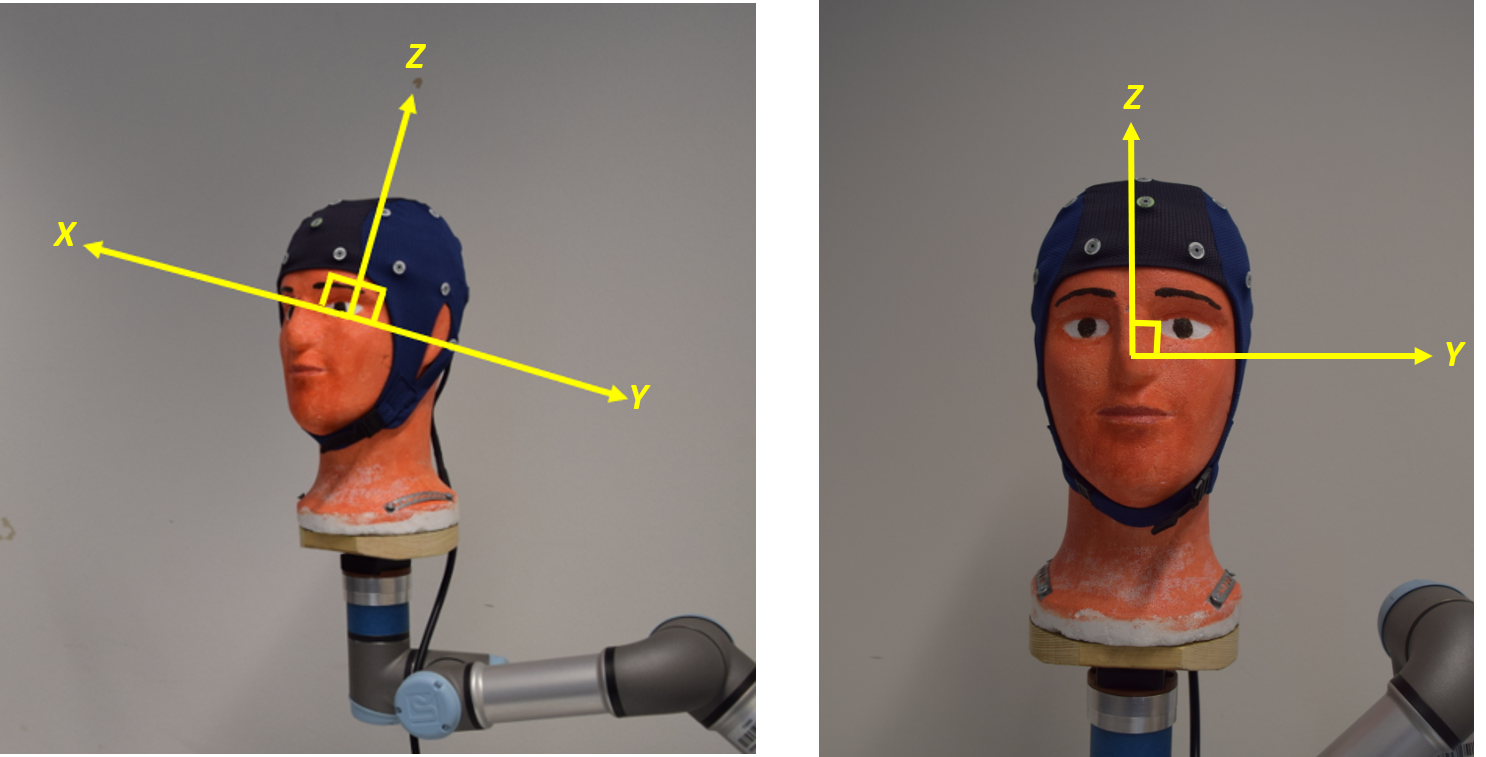
\includegraphics[width=\linewidth]{blue_cap_csys_1.png}
	\caption{Head coordinate system for blue EEG cap} 
	\label{fig:blue_cap_csys}
\end{figure}

\begin{figure}[hbt!]
	\centering
	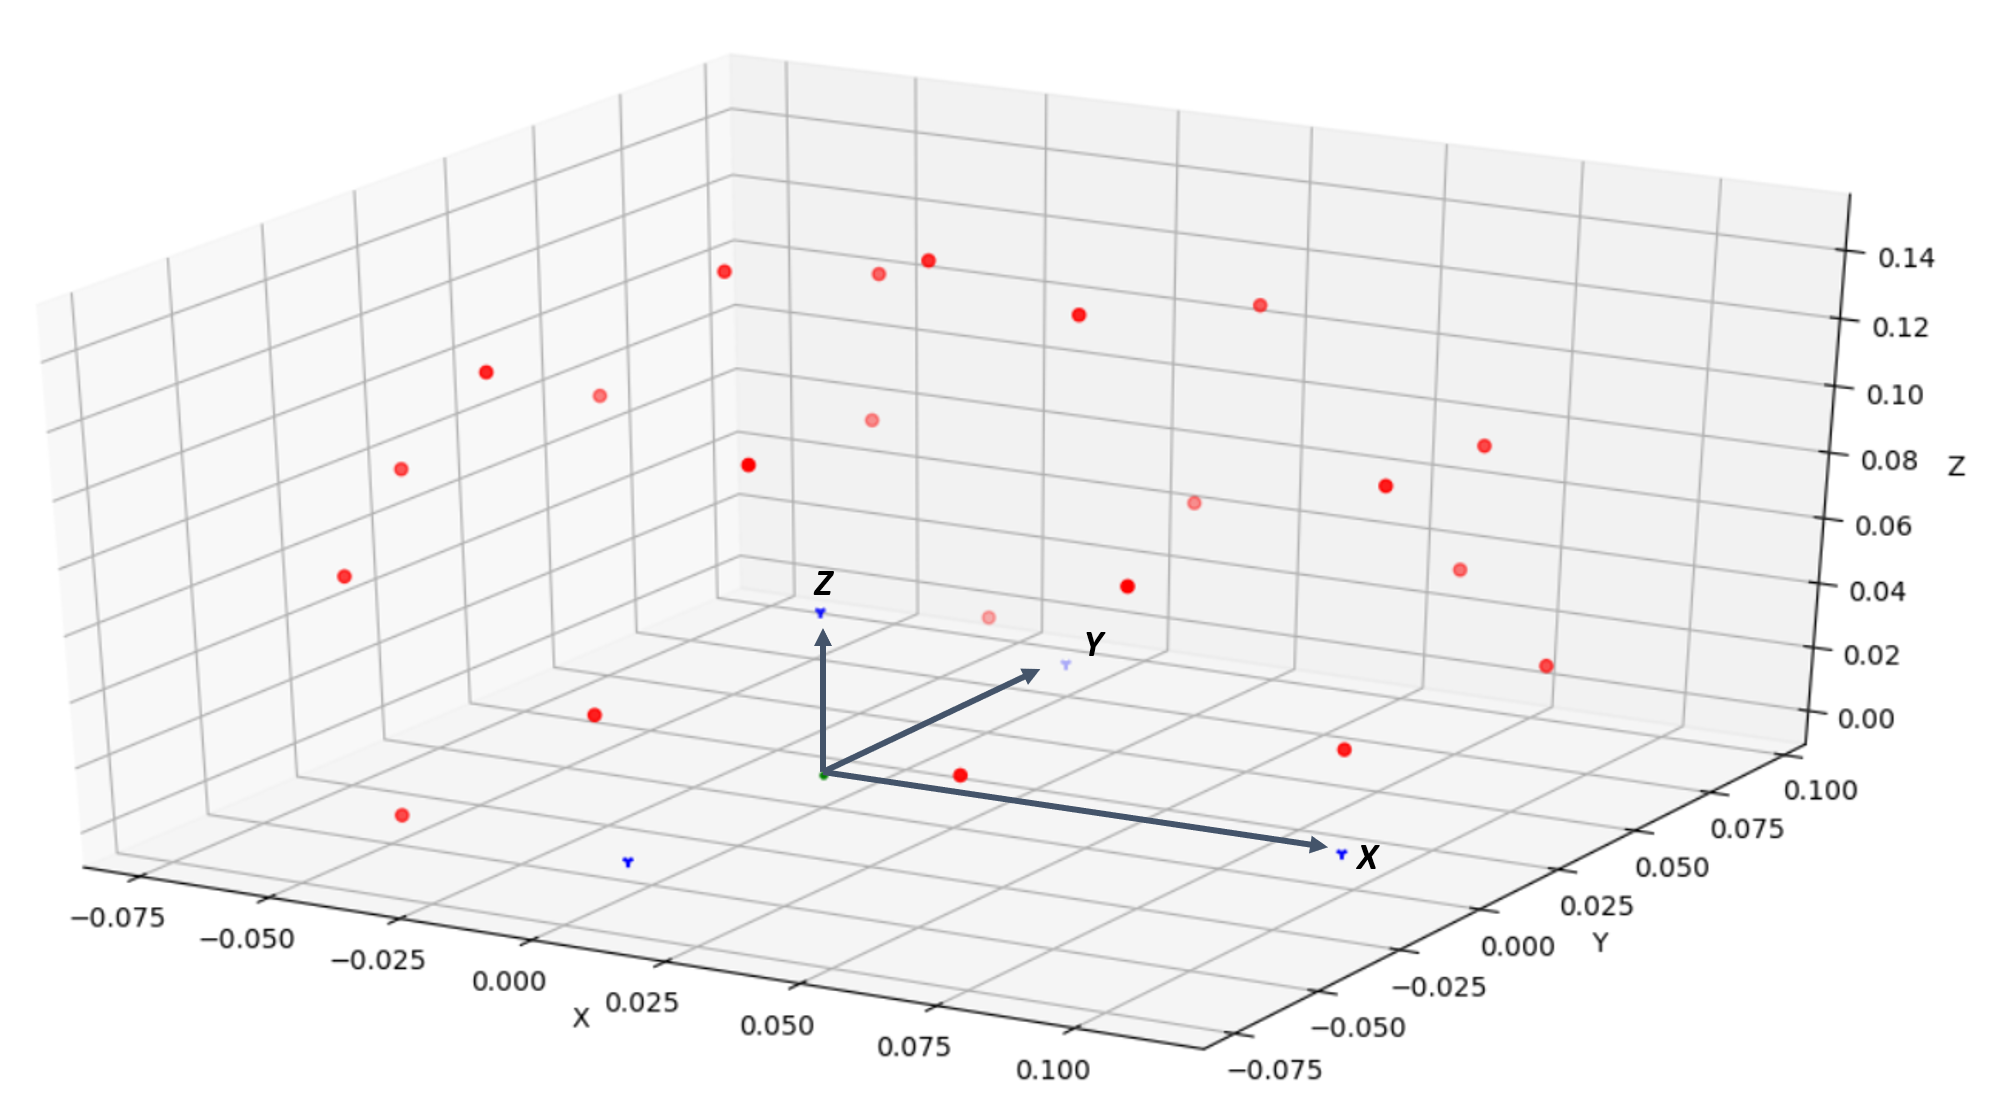
\includegraphics[width=\linewidth]{blue_cap_1.png}
	\caption{All the 22 electrodes are mapped to the head coordinate system} 
	\label{fig:electrodes_blue_cap_1}
\end{figure}

\begin{figure}[hbt!]
	\centering
	\begin{subfigure}{0.49\textwidth}
		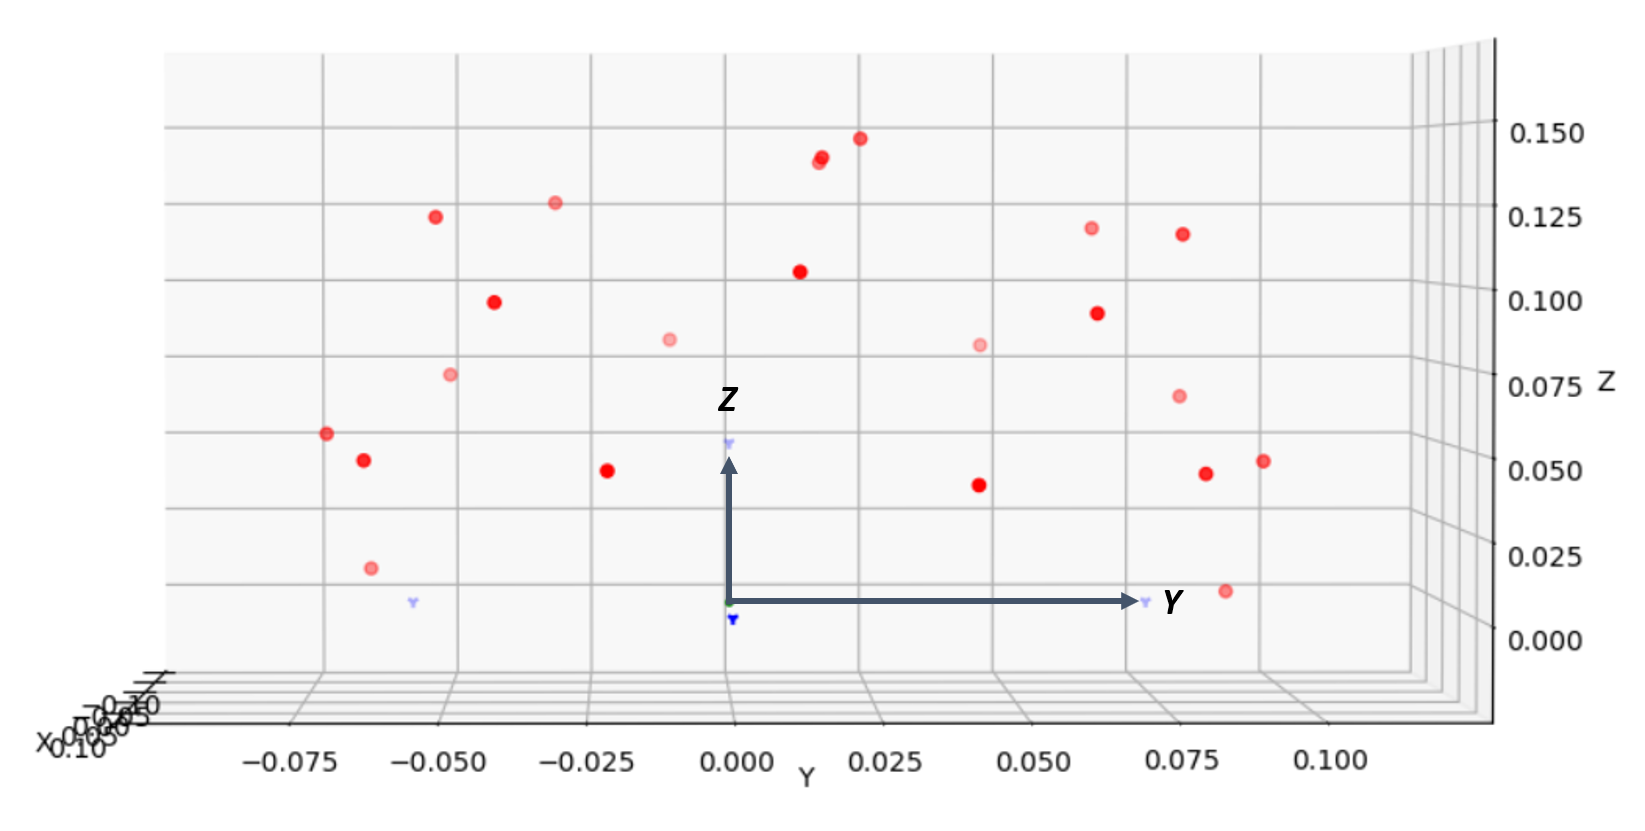
\includegraphics[width=\textwidth]{blue_cap_1_side_view_1.png}	
	\end{subfigure}
	\hfill
	\begin{subfigure}{0.49\textwidth}
		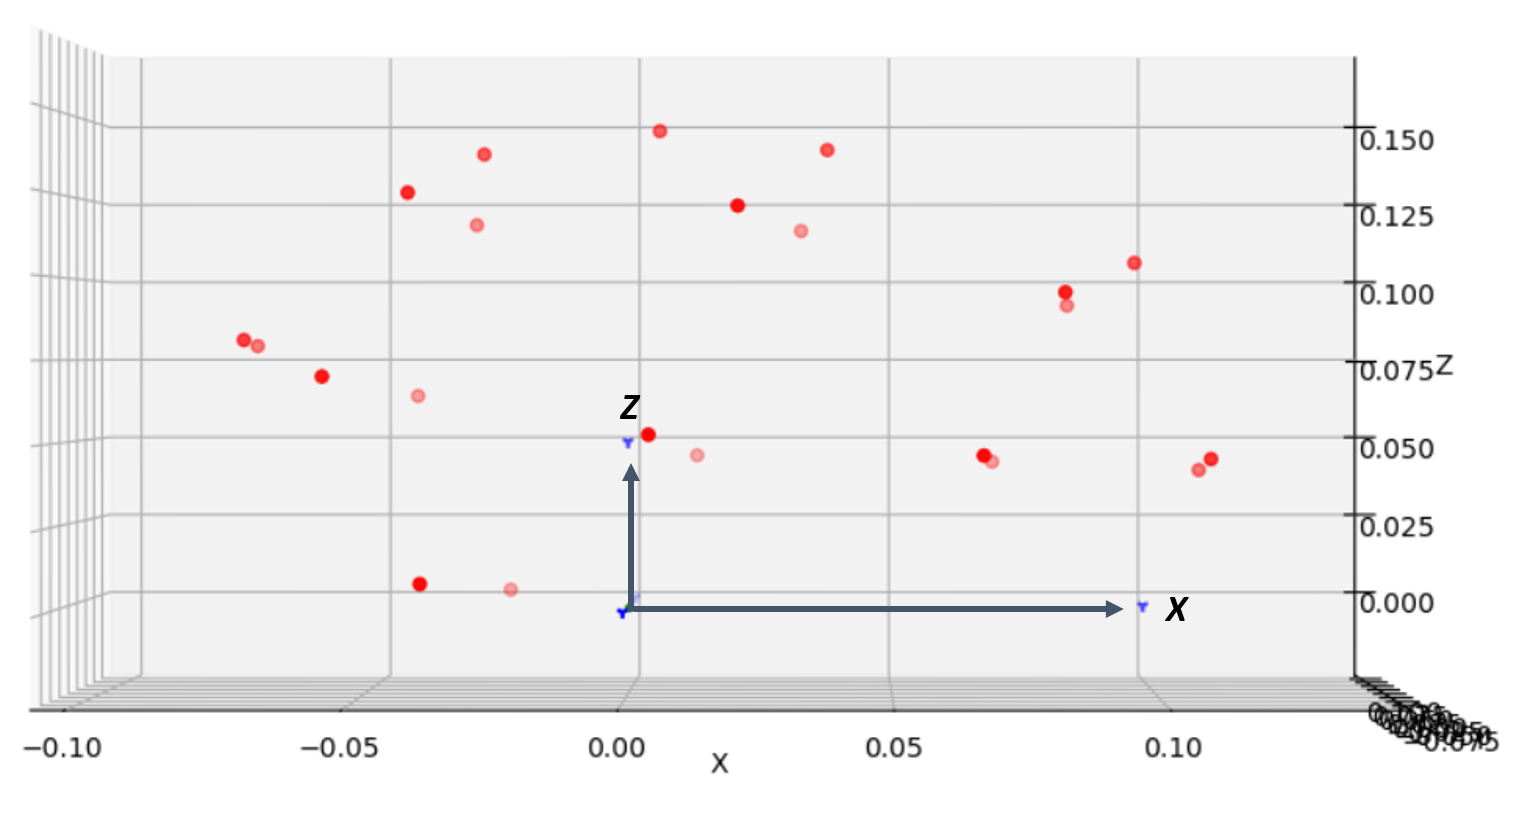
\includegraphics[width=\textwidth]{blue_cap_1_side_view_2.png}	
	\end{subfigure}
	\caption{side views of all 22 electrodes in head coordinate system} 
	\label{fig:electrodes_blue_cap_1_side_view}
\end{figure} 

To evalate how consistance wearing the EEG cap on the patient head, we tried to simulate the attaching the EEG cap for 5 times and measure the variance of the electrode position. \cref{fig:blue_cap_all} shows the electrode position at 5 such instances of attaching the cap to phantom head.

\begin{figure}[hbt!]
	\centering
	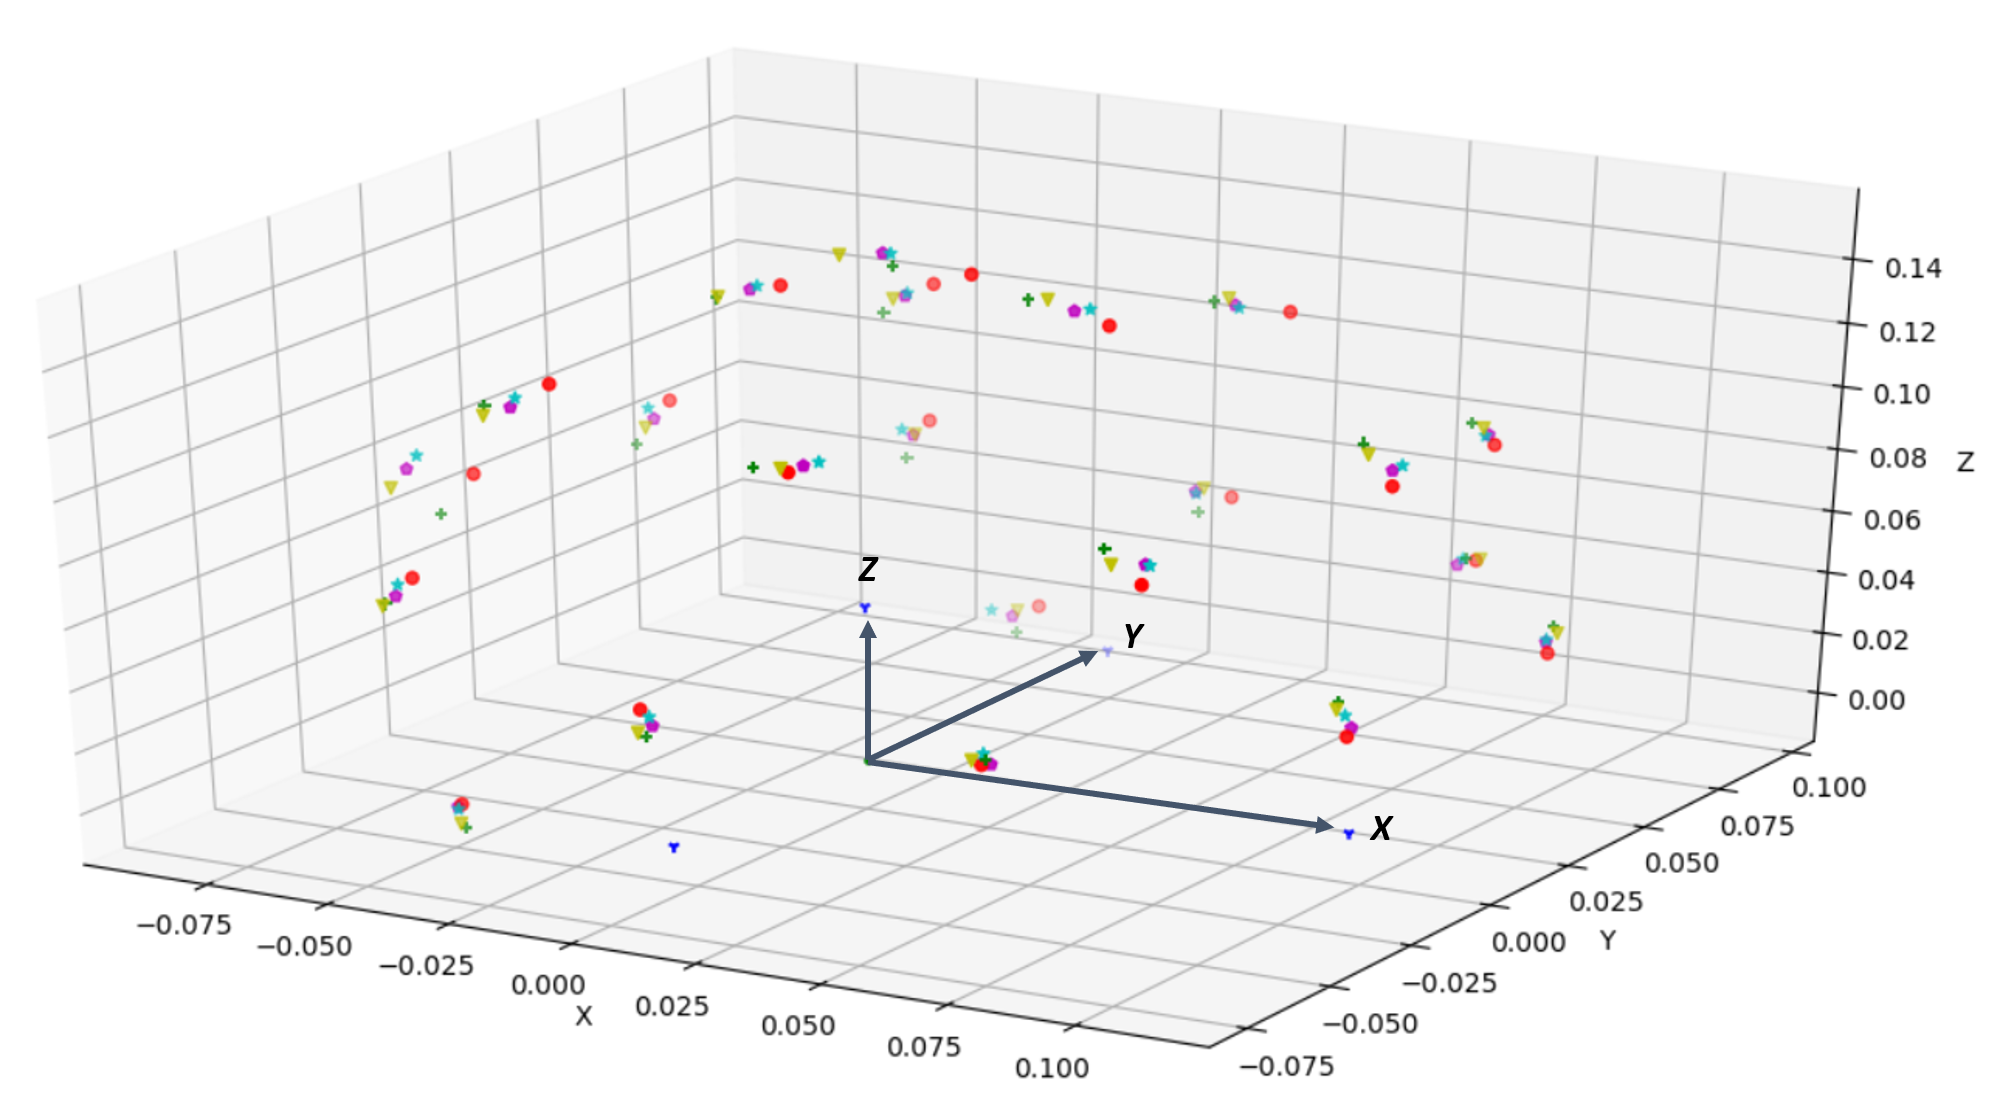
\includegraphics[width=\linewidth]{blue_cap_all.png}
	\caption{electrodes at 5 different EEG cap wearing instances} 
	\label{fig:blue_cap_all}
\end{figure}


\begin{figure}[hbt!]
	\centering
	\begin{subfigure}{0.49\textwidth}
		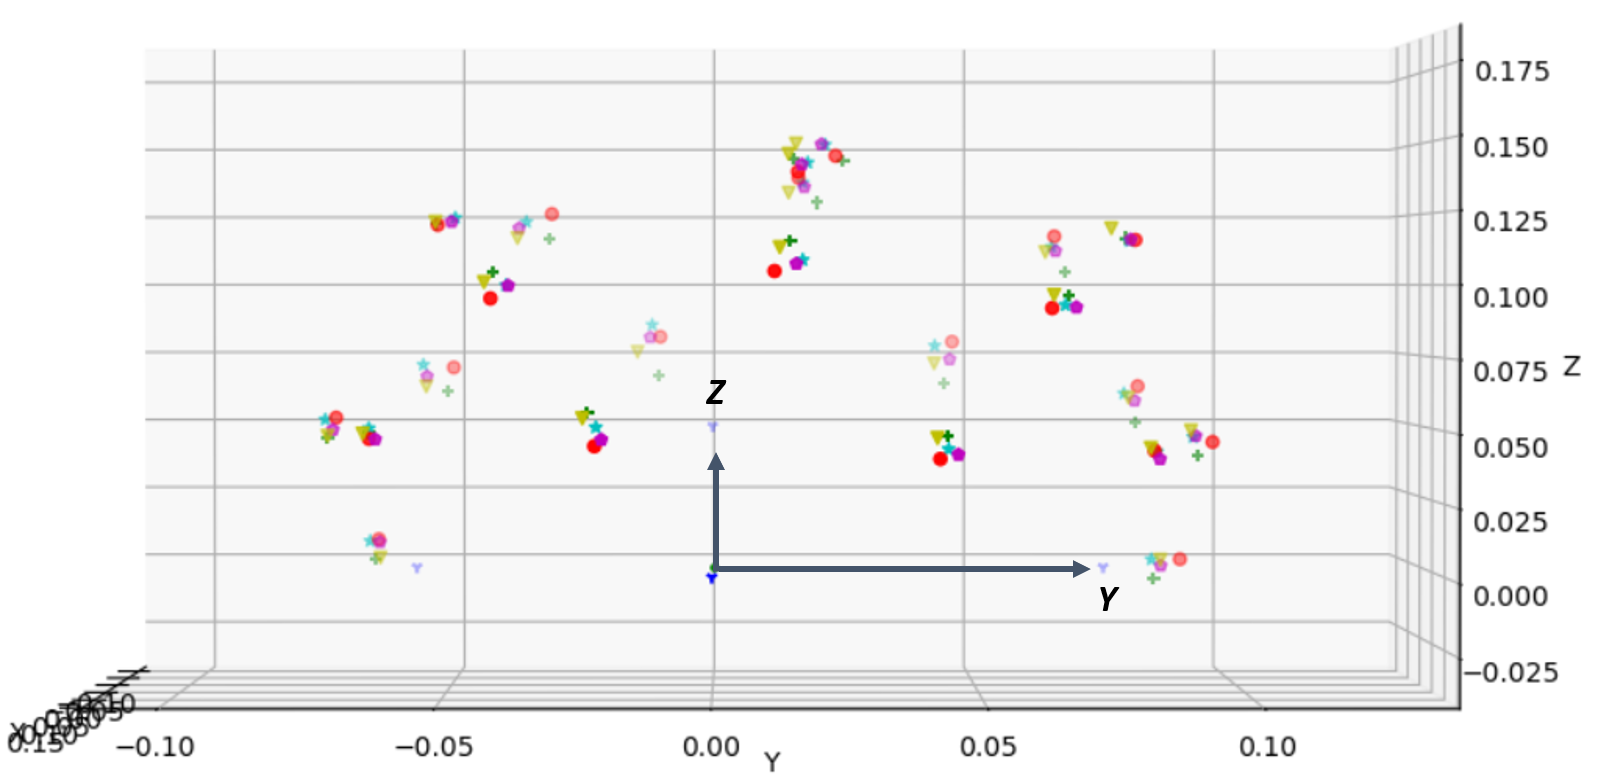
\includegraphics[width=\textwidth]{blue_cap_all_side_view_1.png}	
	\end{subfigure}
	\hfill
	\begin{subfigure}{0.49\textwidth}
		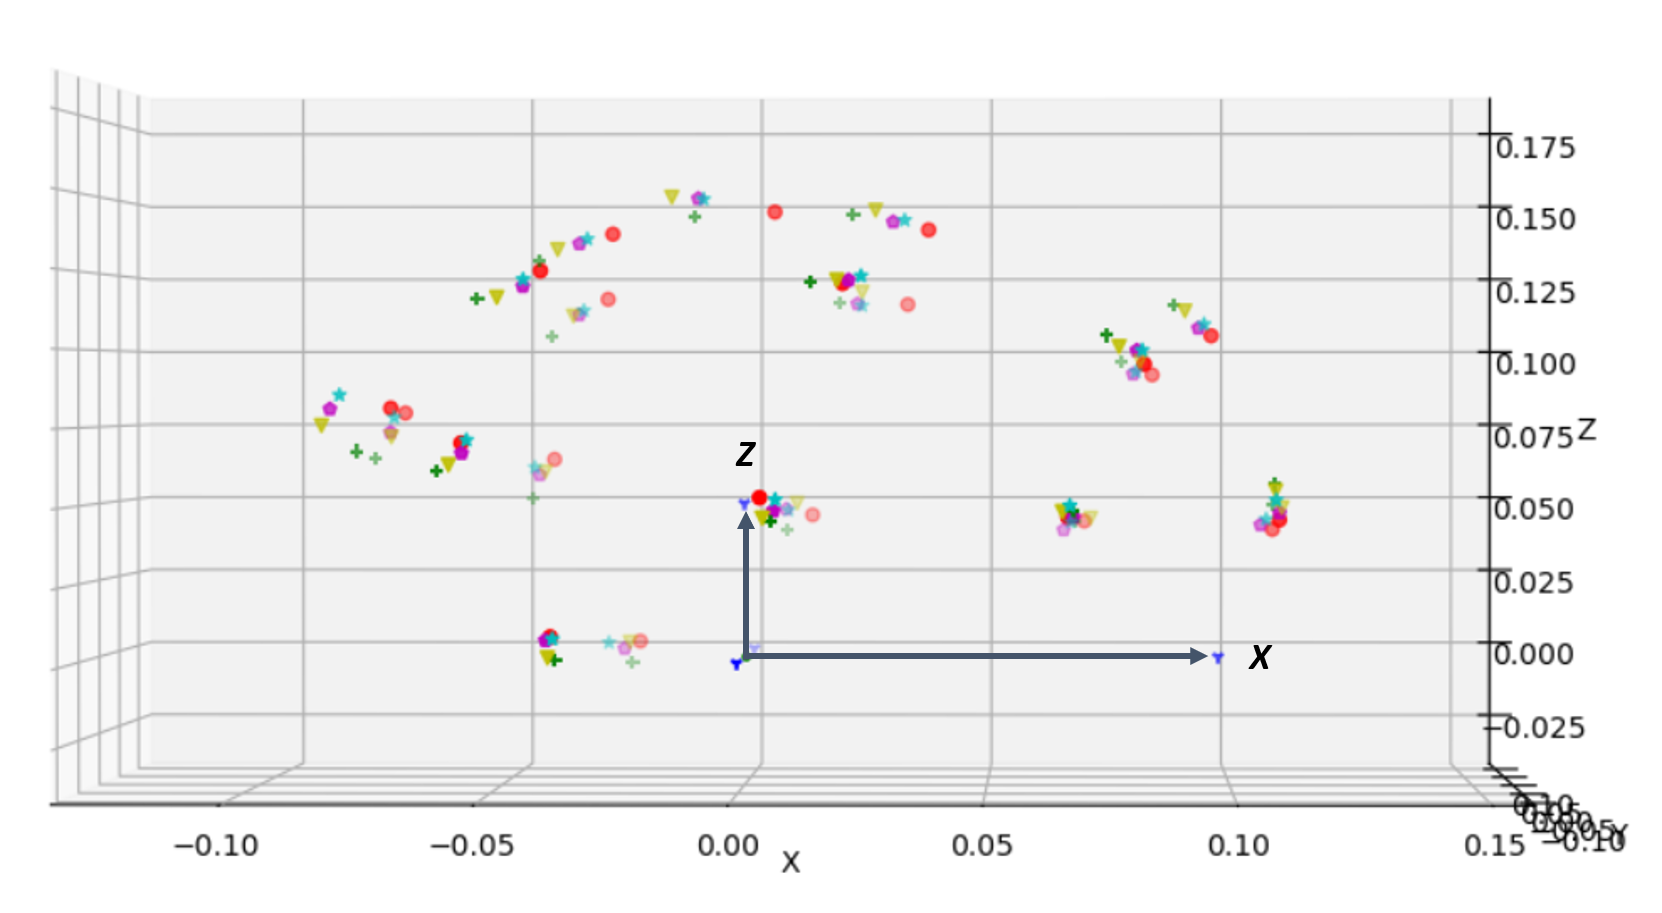
\includegraphics[width=\textwidth]{blue_cap_all_side_view_2.png}	
	\end{subfigure}
	\caption{side views of electrodes at 5 different EEG cap wearing instances} 
	\label{fig:blue_cap_all_side_view}
\end{figure} 

More detailed values of the mean electrode position, standard deviation is provided in the \cref{tab:5x_blue_cap_mean_std}.

\begin{table}[hbt!]
	\centering
	\begin{tabular}{|c|c|c|c|c|c|c|}
		\hline
		Electrode & \multicolumn{2}{c}{x-axis} & \multicolumn{2}{|c}{y-axis} & \multicolumn{2}{|c|}{z-axis} \\ \hline
		Position & mean & SD & mean & SD & mean & SD \\ \hline
		Fp1 & 0.1092 & 0.0015 & 0.0432 & 0.0014 & 0.0448 & 0.0031 \\ 
		Fp2 & 0.1094 & 0.0004 & -0.0219 & 0.0012 & 0.0510 & 0.0043 \\ 
		F7 & 0.0686 & 0.0020 & 0.0827 & 0.0006 & 0.0423 & 0.0014 \\ 
		F3 & 0.0812 & 0.0021 & 0.0652 & 0.0017 & 0.0941 & 0.0020 \\ 
		Fz & 0.0929 & 0.0028 & 0.0142 & 0.0019 & 0.1097 & 0.0037 \\ 
		F4 & 0.0793 & 0.0029 & -0.0400 & 0.0017 & 0.1001 & 0.0030 \\ 
		F8 & 0.0669 & 0.0008 & -0.0641 & 0.0008 & 0.0482 & 0.0014 \\ 
		M1 & -0.0275 & 0.0022 & 0.0865 & 0.0019 & 0.0000 & 0.0026 \\ 
		T3 & 0.0081 & 0.0021 & 0.0925 & 0.0014 & 0.0451 & 0.0031 \\ 
		C3 & 0.0236 & 0.0048 & 0.0785 & 0.0015 & 0.1167 & 0.0016 \\ 
		Cz & 0.0300 & 0.0053 & 0.0162 & 0.0012 & 0.1430 & 0.0022 \\ 
		C4 & 0.0207 & 0.0034 & -0.0511 & 0.0017 & 0.1221 & 0.0008 \\ 
		T4 & 0.0068 & 0.0012 & -0.0730 & 0.0007 & 0.0494 & 0.0030 \\ 
		M2 & -0.0372 & 0.0007 & -0.0652 & 0.0007 & 0.0056 & 0.0031 \\ 
		T5 & -0.0456 & 0.0017 & 0.0813 & 0.0010 & 0.0585 & 0.0045 \\ 
		P3 & -0.0369 & 0.0038 & 0.0661 & 0.0013 & 0.1119 & 0.0041 \\ 
		Pz & -0.0356 & 0.0053 & 0.0172 & 0.0018 & 0.1345 & 0.0030 \\ 
		P4 & -0.0462 & 0.0045 & -0.0350 & 0.0029 & 0.1203 & 0.0034 \\ 
		T6 & -0.0569 & 0.0022 & -0.0542 & 0.0024 & 0.0666 & 0.0038 \\ 
		O1 & -0.0755 & 0.0020 & 0.0450 & 0.0015 & 0.0732 & 0.0053 \\ 
		O2 & -0.0811 & 0.0050 & -0.0122 & 0.0016 & 0.0780 & 0.0063 \\ 
		REF & -0.0080 & 0.0072 & 0.0213 & 0.0031 & 0.1480 & 0.0026 \\ 
		\hline
	\end{tabular}
	\caption{Data of electrode mean position, standard deviation for 5 different EEG cap wearing instances}
	\label{tab:5x_blue_cap_mean_std}
\end{table}



